% Created by tikzDevice version 0.12.6 on 2024-02-26 22:01:36
% !TEX encoding = UTF-8 Unicode
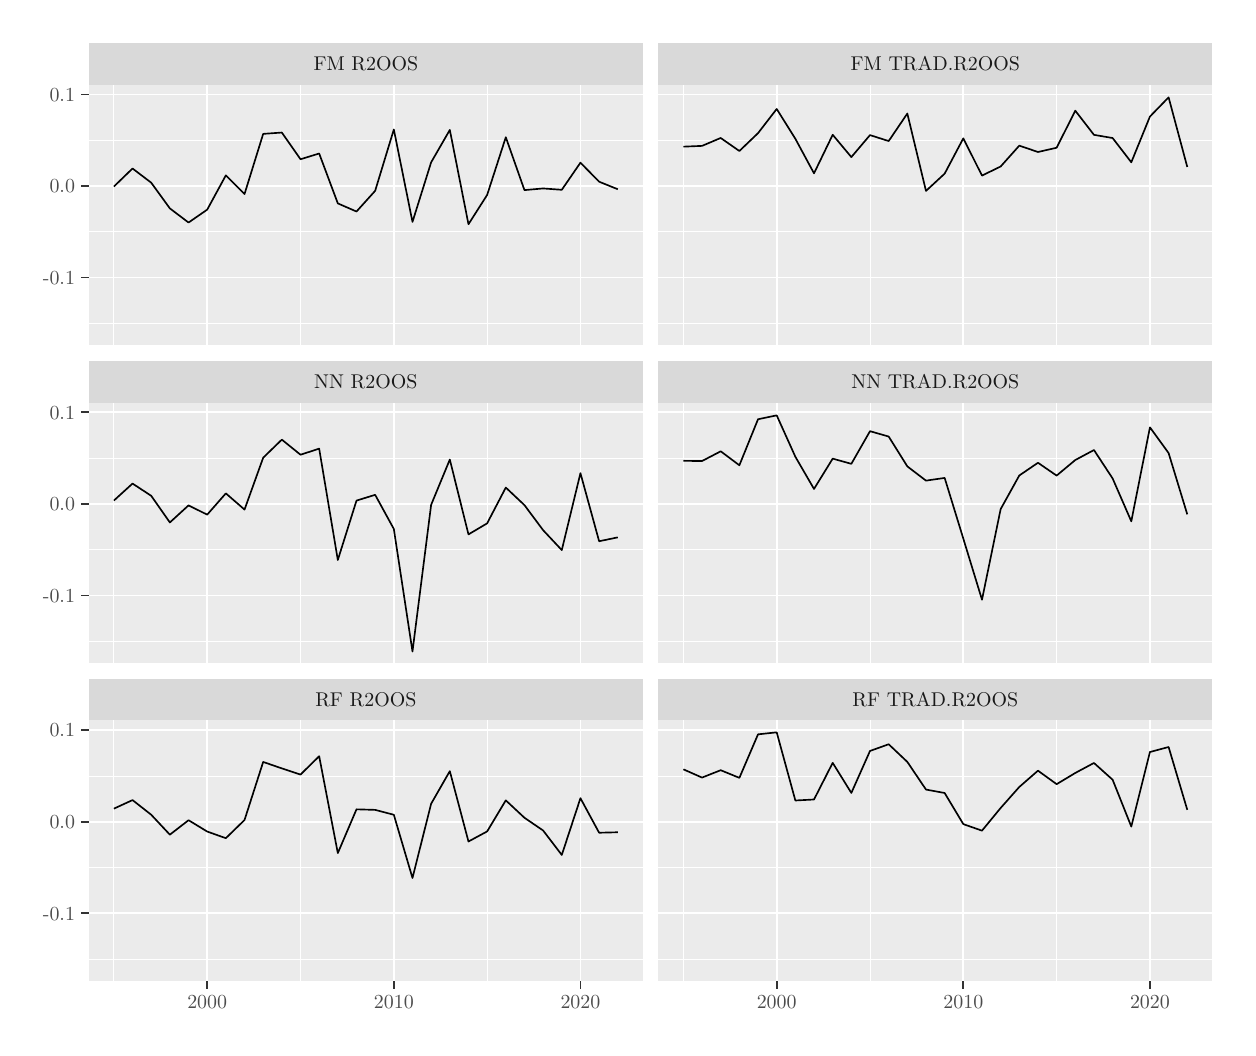
\begin{tikzpicture}[x=1pt,y=1pt]
\definecolor{fillColor}{RGB}{255,255,255}
\path[use as bounding box,fill=fillColor,fill opacity=0.00] (0,0) rectangle (433.62,361.35);
\begin{scope}
\path[clip] (  0.00,  0.00) rectangle (433.62,361.35);
\definecolor{drawColor}{RGB}{255,255,255}
\definecolor{fillColor}{RGB}{255,255,255}

\path[draw=drawColor,line width= 0.6pt,line join=round,line cap=round,fill=fillColor] (  0.00,  0.00) rectangle (433.62,361.35);
\end{scope}
\begin{scope}
\path[clip] ( 22.05,246.50) rectangle (222.33,340.69);
\definecolor{fillColor}{gray}{0.92}

\path[fill=fillColor] ( 22.05,246.50) rectangle (222.33,340.69);
\definecolor{drawColor}{RGB}{255,255,255}

\path[draw=drawColor,line width= 0.3pt,line join=round] ( 22.05,254.47) --
	(222.33,254.47);

\path[draw=drawColor,line width= 0.3pt,line join=round] ( 22.05,287.57) --
	(222.33,287.57);

\path[draw=drawColor,line width= 0.3pt,line join=round] ( 22.05,320.67) --
	(222.33,320.67);

\path[draw=drawColor,line width= 0.3pt,line join=round] ( 31.15,246.50) --
	( 31.15,340.69);

\path[draw=drawColor,line width= 0.3pt,line join=round] ( 98.59,246.50) --
	( 98.59,340.69);

\path[draw=drawColor,line width= 0.3pt,line join=round] (166.02,246.50) --
	(166.02,340.69);

\path[draw=drawColor,line width= 0.6pt,line join=round] ( 22.05,271.02) --
	(222.33,271.02);

\path[draw=drawColor,line width= 0.6pt,line join=round] ( 22.05,304.12) --
	(222.33,304.12);

\path[draw=drawColor,line width= 0.6pt,line join=round] ( 22.05,337.21) --
	(222.33,337.21);

\path[draw=drawColor,line width= 0.6pt,line join=round] ( 64.87,246.50) --
	( 64.87,340.69);

\path[draw=drawColor,line width= 0.6pt,line join=round] (132.31,246.50) --
	(132.31,340.69);

\path[draw=drawColor,line width= 0.6pt,line join=round] (199.74,246.50) --
	(199.74,340.69);
\definecolor{drawColor}{RGB}{0,0,0}

\path[draw=drawColor,line width= 0.6pt,line join=round] ( 31.15,303.93) --
	( 37.89,310.46) --
	( 44.64,305.33) --
	( 51.38,296.04) --
	( 58.13,290.93) --
	( 64.87,295.59) --
	( 71.61,307.98) --
	( 78.36,301.23) --
	( 85.10,322.97) --
	( 91.84,323.45) --
	( 98.59,313.80) --
	(105.33,315.88) --
	(112.07,297.85) --
	(118.82,294.91) --
	(125.56,302.39) --
	(132.31,324.56) --
	(139.05,291.16) --
	(145.79,312.69) --
	(152.54,324.40) --
	(159.28,290.32) --
	(166.02,300.89) --
	(172.77,321.76) --
	(179.51,302.65) --
	(186.26,303.25) --
	(193.00,302.76) --
	(199.74,312.56) --
	(206.49,305.69) --
	(213.23,302.96);
\end{scope}
\begin{scope}
\path[clip] ( 22.05,131.66) rectangle (222.33,225.84);
\definecolor{fillColor}{gray}{0.92}

\path[fill=fillColor] ( 22.05,131.66) rectangle (222.33,225.84);
\definecolor{drawColor}{RGB}{255,255,255}

\path[draw=drawColor,line width= 0.3pt,line join=round] ( 22.05,139.63) --
	(222.33,139.63);

\path[draw=drawColor,line width= 0.3pt,line join=round] ( 22.05,172.72) --
	(222.33,172.72);

\path[draw=drawColor,line width= 0.3pt,line join=round] ( 22.05,205.82) --
	(222.33,205.82);

\path[draw=drawColor,line width= 0.3pt,line join=round] ( 31.15,131.66) --
	( 31.15,225.84);

\path[draw=drawColor,line width= 0.3pt,line join=round] ( 98.59,131.66) --
	( 98.59,225.84);

\path[draw=drawColor,line width= 0.3pt,line join=round] (166.02,131.66) --
	(166.02,225.84);

\path[draw=drawColor,line width= 0.6pt,line join=round] ( 22.05,156.17) --
	(222.33,156.17);

\path[draw=drawColor,line width= 0.6pt,line join=round] ( 22.05,189.27) --
	(222.33,189.27);

\path[draw=drawColor,line width= 0.6pt,line join=round] ( 22.05,222.37) --
	(222.33,222.37);

\path[draw=drawColor,line width= 0.6pt,line join=round] ( 64.87,131.66) --
	( 64.87,225.84);

\path[draw=drawColor,line width= 0.6pt,line join=round] (132.31,131.66) --
	(132.31,225.84);

\path[draw=drawColor,line width= 0.6pt,line join=round] (199.74,131.66) --
	(199.74,225.84);
\definecolor{drawColor}{RGB}{0,0,0}

\path[draw=drawColor,line width= 0.6pt,line join=round] ( 31.15,190.47) --
	( 37.89,196.61) --
	( 44.64,192.19) --
	( 51.38,182.56) --
	( 58.13,188.73) --
	( 64.87,185.38) --
	( 71.61,193.07) --
	( 78.36,187.21) --
	( 85.10,205.95) --
	( 91.84,212.49) --
	( 98.59,207.03) --
	(105.33,209.23) --
	(112.07,169.00) --
	(118.82,190.46) --
	(125.56,192.54) --
	(132.31,180.21) --
	(139.05,135.94) --
	(145.79,188.93) --
	(152.54,205.29) --
	(159.28,178.24) --
	(166.02,182.23) --
	(172.77,195.17) --
	(179.51,188.82) --
	(186.26,179.76) --
	(193.00,172.57) --
	(199.74,200.38) --
	(206.49,175.77) --
	(213.23,177.17);
\end{scope}
\begin{scope}
\path[clip] ( 22.05, 16.81) rectangle (222.33,111.00);
\definecolor{fillColor}{gray}{0.92}

\path[fill=fillColor] ( 22.05, 16.81) rectangle (222.33,111.00);
\definecolor{drawColor}{RGB}{255,255,255}

\path[draw=drawColor,line width= 0.3pt,line join=round] ( 22.05, 24.78) --
	(222.33, 24.78);

\path[draw=drawColor,line width= 0.3pt,line join=round] ( 22.05, 57.88) --
	(222.33, 57.88);

\path[draw=drawColor,line width= 0.3pt,line join=round] ( 22.05, 90.97) --
	(222.33, 90.97);

\path[draw=drawColor,line width= 0.3pt,line join=round] ( 31.15, 16.81) --
	( 31.15,111.00);

\path[draw=drawColor,line width= 0.3pt,line join=round] ( 98.59, 16.81) --
	( 98.59,111.00);

\path[draw=drawColor,line width= 0.3pt,line join=round] (166.02, 16.81) --
	(166.02,111.00);

\path[draw=drawColor,line width= 0.6pt,line join=round] ( 22.05, 41.33) --
	(222.33, 41.33);

\path[draw=drawColor,line width= 0.6pt,line join=round] ( 22.05, 74.42) --
	(222.33, 74.42);

\path[draw=drawColor,line width= 0.6pt,line join=round] ( 22.05,107.52) --
	(222.33,107.52);

\path[draw=drawColor,line width= 0.6pt,line join=round] ( 64.87, 16.81) --
	( 64.87,111.00);

\path[draw=drawColor,line width= 0.6pt,line join=round] (132.31, 16.81) --
	(132.31,111.00);

\path[draw=drawColor,line width= 0.6pt,line join=round] (199.74, 16.81) --
	(199.74,111.00);
\definecolor{drawColor}{RGB}{0,0,0}

\path[draw=drawColor,line width= 0.6pt,line join=round] ( 31.15, 79.14) --
	( 37.89, 82.24) --
	( 44.64, 76.94) --
	( 51.38, 69.74) --
	( 58.13, 74.97) --
	( 64.87, 70.87) --
	( 71.61, 68.47) --
	( 78.36, 75.04) --
	( 85.10, 96.02) --
	( 91.84, 93.69) --
	( 98.59, 91.46) --
	(105.33, 98.09) --
	(112.07, 63.08) --
	(118.82, 78.90) --
	(125.56, 78.70) --
	(132.31, 76.93) --
	(139.05, 54.09) --
	(145.79, 80.92) --
	(152.54, 92.70) --
	(159.28, 67.27) --
	(166.02, 70.91) --
	(172.77, 82.14) --
	(179.51, 75.85) --
	(186.26, 71.24) --
	(193.00, 62.41) --
	(199.74, 82.92) --
	(206.49, 70.44) --
	(213.23, 70.61);
\end{scope}
\begin{scope}
\path[clip] (227.83,246.50) rectangle (428.12,340.69);
\definecolor{fillColor}{gray}{0.92}

\path[fill=fillColor] (227.83,246.50) rectangle (428.12,340.69);
\definecolor{drawColor}{RGB}{255,255,255}

\path[draw=drawColor,line width= 0.3pt,line join=round] (227.83,254.47) --
	(428.12,254.47);

\path[draw=drawColor,line width= 0.3pt,line join=round] (227.83,287.57) --
	(428.12,287.57);

\path[draw=drawColor,line width= 0.3pt,line join=round] (227.83,320.67) --
	(428.12,320.67);

\path[draw=drawColor,line width= 0.3pt,line join=round] (236.94,246.50) --
	(236.94,340.69);

\path[draw=drawColor,line width= 0.3pt,line join=round] (304.37,246.50) --
	(304.37,340.69);

\path[draw=drawColor,line width= 0.3pt,line join=round] (371.81,246.50) --
	(371.81,340.69);

\path[draw=drawColor,line width= 0.6pt,line join=round] (227.83,271.02) --
	(428.12,271.02);

\path[draw=drawColor,line width= 0.6pt,line join=round] (227.83,304.12) --
	(428.12,304.12);

\path[draw=drawColor,line width= 0.6pt,line join=round] (227.83,337.21) --
	(428.12,337.21);

\path[draw=drawColor,line width= 0.6pt,line join=round] (270.66,246.50) --
	(270.66,340.69);

\path[draw=drawColor,line width= 0.6pt,line join=round] (338.09,246.50) --
	(338.09,340.69);

\path[draw=drawColor,line width= 0.6pt,line join=round] (405.53,246.50) --
	(405.53,340.69);
\definecolor{drawColor}{RGB}{0,0,0}

\path[draw=drawColor,line width= 0.6pt,line join=round] (236.94,318.35) --
	(243.68,318.63) --
	(250.42,321.49) --
	(257.17,316.78) --
	(263.91,323.23) --
	(270.66,331.97) --
	(277.40,321.20) --
	(284.14,308.71) --
	(290.89,322.64) --
	(297.63,314.58) --
	(304.37,322.53) --
	(311.12,320.37) --
	(317.86,330.32) --
	(324.60,302.35) --
	(331.35,308.60) --
	(338.09,321.36) --
	(344.84,307.90) --
	(351.58,311.18) --
	(358.32,318.72) --
	(365.07,316.42) --
	(371.81,317.96) --
	(378.55,331.35) --
	(385.30,322.62) --
	(392.04,321.47) --
	(398.79,312.70) --
	(405.53,329.24) --
	(412.27,336.16) --
	(419.02,311.01);
\end{scope}
\begin{scope}
\path[clip] (227.83,131.66) rectangle (428.12,225.84);
\definecolor{fillColor}{gray}{0.92}

\path[fill=fillColor] (227.83,131.66) rectangle (428.12,225.84);
\definecolor{drawColor}{RGB}{255,255,255}

\path[draw=drawColor,line width= 0.3pt,line join=round] (227.83,139.63) --
	(428.12,139.63);

\path[draw=drawColor,line width= 0.3pt,line join=round] (227.83,172.72) --
	(428.12,172.72);

\path[draw=drawColor,line width= 0.3pt,line join=round] (227.83,205.82) --
	(428.12,205.82);

\path[draw=drawColor,line width= 0.3pt,line join=round] (236.94,131.66) --
	(236.94,225.84);

\path[draw=drawColor,line width= 0.3pt,line join=round] (304.37,131.66) --
	(304.37,225.84);

\path[draw=drawColor,line width= 0.3pt,line join=round] (371.81,131.66) --
	(371.81,225.84);

\path[draw=drawColor,line width= 0.6pt,line join=round] (227.83,156.17) --
	(428.12,156.17);

\path[draw=drawColor,line width= 0.6pt,line join=round] (227.83,189.27) --
	(428.12,189.27);

\path[draw=drawColor,line width= 0.6pt,line join=round] (227.83,222.37) --
	(428.12,222.37);

\path[draw=drawColor,line width= 0.6pt,line join=round] (270.66,131.66) --
	(270.66,225.84);

\path[draw=drawColor,line width= 0.6pt,line join=round] (338.09,131.66) --
	(338.09,225.84);

\path[draw=drawColor,line width= 0.6pt,line join=round] (405.53,131.66) --
	(405.53,225.84);
\definecolor{drawColor}{RGB}{0,0,0}

\path[draw=drawColor,line width= 0.6pt,line join=round] (236.94,204.83) --
	(243.68,204.75) --
	(250.42,208.27) --
	(257.17,203.22) --
	(263.91,219.85) --
	(270.66,221.26) --
	(277.40,206.30) --
	(284.14,194.67) --
	(290.89,205.62) --
	(297.63,203.74) --
	(304.37,215.54) --
	(311.12,213.60) --
	(317.86,202.82) --
	(324.60,197.67) --
	(331.35,198.65) --
	(338.09,176.71) --
	(344.84,154.64) --
	(351.58,187.38) --
	(358.32,199.53) --
	(365.07,204.13) --
	(371.81,199.49) --
	(378.55,205.12) --
	(385.30,208.73) --
	(392.04,198.46) --
	(398.79,182.97) --
	(405.53,216.93) --
	(412.27,207.63) --
	(419.02,185.48);
\end{scope}
\begin{scope}
\path[clip] (227.83, 16.81) rectangle (428.12,111.00);
\definecolor{fillColor}{gray}{0.92}

\path[fill=fillColor] (227.83, 16.81) rectangle (428.12,111.00);
\definecolor{drawColor}{RGB}{255,255,255}

\path[draw=drawColor,line width= 0.3pt,line join=round] (227.83, 24.78) --
	(428.12, 24.78);

\path[draw=drawColor,line width= 0.3pt,line join=round] (227.83, 57.88) --
	(428.12, 57.88);

\path[draw=drawColor,line width= 0.3pt,line join=round] (227.83, 90.97) --
	(428.12, 90.97);

\path[draw=drawColor,line width= 0.3pt,line join=round] (236.94, 16.81) --
	(236.94,111.00);

\path[draw=drawColor,line width= 0.3pt,line join=round] (304.37, 16.81) --
	(304.37,111.00);

\path[draw=drawColor,line width= 0.3pt,line join=round] (371.81, 16.81) --
	(371.81,111.00);

\path[draw=drawColor,line width= 0.6pt,line join=round] (227.83, 41.33) --
	(428.12, 41.33);

\path[draw=drawColor,line width= 0.6pt,line join=round] (227.83, 74.42) --
	(428.12, 74.42);

\path[draw=drawColor,line width= 0.6pt,line join=round] (227.83,107.52) --
	(428.12,107.52);

\path[draw=drawColor,line width= 0.6pt,line join=round] (270.66, 16.81) --
	(270.66,111.00);

\path[draw=drawColor,line width= 0.6pt,line join=round] (338.09, 16.81) --
	(338.09,111.00);

\path[draw=drawColor,line width= 0.6pt,line join=round] (405.53, 16.81) --
	(405.53,111.00);
\definecolor{drawColor}{RGB}{0,0,0}

\path[draw=drawColor,line width= 0.6pt,line join=round] (236.94, 93.35) --
	(243.68, 90.37) --
	(250.42, 93.04) --
	(257.17, 90.27) --
	(263.91,105.99) --
	(270.66,106.72) --
	(277.40, 82.09) --
	(284.14, 82.45) --
	(290.89, 95.69) --
	(297.63, 84.82) --
	(304.37, 99.99) --
	(311.12,102.41) --
	(317.86, 96.04) --
	(324.60, 86.04) --
	(331.35, 84.80) --
	(338.09, 73.55) --
	(344.84, 71.19) --
	(351.58, 79.39) --
	(358.32, 86.98) --
	(365.07, 92.87) --
	(371.81, 87.99) --
	(378.55, 92.04) --
	(385.30, 95.65) --
	(392.04, 89.59) --
	(398.79, 72.67) --
	(405.53, 99.61) --
	(412.27,101.42) --
	(419.02, 78.72);
\end{scope}
\begin{scope}
\path[clip] ( 22.05,111.00) rectangle (222.33,126.16);
\definecolor{fillColor}{gray}{0.85}

\path[fill=fillColor] ( 22.05,111.00) rectangle (222.33,126.16);
\definecolor{drawColor}{gray}{0.10}

\node[text=drawColor,anchor=base,inner sep=0pt, outer sep=0pt, scale=  0.72] at (122.19,116.10) {RF R2OOS};
\end{scope}
\begin{scope}
\path[clip] (227.83,111.00) rectangle (428.12,126.16);
\definecolor{fillColor}{gray}{0.85}

\path[fill=fillColor] (227.83,111.00) rectangle (428.12,126.16);
\definecolor{drawColor}{gray}{0.10}

\node[text=drawColor,anchor=base,inner sep=0pt, outer sep=0pt, scale=  0.72] at (327.98,116.10) {RF TRAD.R2OOS};
\end{scope}
\begin{scope}
\path[clip] ( 22.05,225.84) rectangle (222.33,241.00);
\definecolor{fillColor}{gray}{0.85}

\path[fill=fillColor] ( 22.05,225.84) rectangle (222.33,241.00);
\definecolor{drawColor}{gray}{0.10}

\node[text=drawColor,anchor=base,inner sep=0pt, outer sep=0pt, scale=  0.72] at (122.19,230.94) {NN R2OOS};
\end{scope}
\begin{scope}
\path[clip] (227.83,225.84) rectangle (428.12,241.00);
\definecolor{fillColor}{gray}{0.85}

\path[fill=fillColor] (227.83,225.84) rectangle (428.12,241.00);
\definecolor{drawColor}{gray}{0.10}

\node[text=drawColor,anchor=base,inner sep=0pt, outer sep=0pt, scale=  0.72] at (327.98,230.94) {NN TRAD.R2OOS};
\end{scope}
\begin{scope}
\path[clip] ( 22.05,340.69) rectangle (222.33,355.85);
\definecolor{fillColor}{gray}{0.85}

\path[fill=fillColor] ( 22.05,340.69) rectangle (222.33,355.85);
\definecolor{drawColor}{gray}{0.10}

\node[text=drawColor,anchor=base,inner sep=0pt, outer sep=0pt, scale=  0.72] at (122.19,345.79) {FM R2OOS};
\end{scope}
\begin{scope}
\path[clip] (227.83,340.69) rectangle (428.12,355.85);
\definecolor{fillColor}{gray}{0.85}

\path[fill=fillColor] (227.83,340.69) rectangle (428.12,355.85);
\definecolor{drawColor}{gray}{0.10}

\node[text=drawColor,anchor=base,inner sep=0pt, outer sep=0pt, scale=  0.72] at (327.98,345.79) {FM TRAD.R2OOS};
\end{scope}
\begin{scope}
\path[clip] (  0.00,  0.00) rectangle (433.62,361.35);
\definecolor{drawColor}{gray}{0.20}

\path[draw=drawColor,line width= 0.6pt,line join=round] ( 64.87, 14.06) --
	( 64.87, 16.81);

\path[draw=drawColor,line width= 0.6pt,line join=round] (132.31, 14.06) --
	(132.31, 16.81);

\path[draw=drawColor,line width= 0.6pt,line join=round] (199.74, 14.06) --
	(199.74, 16.81);
\end{scope}
\begin{scope}
\path[clip] (  0.00,  0.00) rectangle (433.62,361.35);
\definecolor{drawColor}{gray}{0.30}

\node[text=drawColor,anchor=base,inner sep=0pt, outer sep=0pt, scale=  0.72] at ( 64.87,  6.90) {2000};

\node[text=drawColor,anchor=base,inner sep=0pt, outer sep=0pt, scale=  0.72] at (132.31,  6.90) {2010};

\node[text=drawColor,anchor=base,inner sep=0pt, outer sep=0pt, scale=  0.72] at (199.74,  6.90) {2020};
\end{scope}
\begin{scope}
\path[clip] (  0.00,  0.00) rectangle (433.62,361.35);
\definecolor{drawColor}{gray}{0.20}

\path[draw=drawColor,line width= 0.6pt,line join=round] (270.66, 14.06) --
	(270.66, 16.81);

\path[draw=drawColor,line width= 0.6pt,line join=round] (338.09, 14.06) --
	(338.09, 16.81);

\path[draw=drawColor,line width= 0.6pt,line join=round] (405.53, 14.06) --
	(405.53, 16.81);
\end{scope}
\begin{scope}
\path[clip] (  0.00,  0.00) rectangle (433.62,361.35);
\definecolor{drawColor}{gray}{0.30}

\node[text=drawColor,anchor=base,inner sep=0pt, outer sep=0pt, scale=  0.72] at (270.66,  6.90) {2000};

\node[text=drawColor,anchor=base,inner sep=0pt, outer sep=0pt, scale=  0.72] at (338.09,  6.90) {2010};

\node[text=drawColor,anchor=base,inner sep=0pt, outer sep=0pt, scale=  0.72] at (405.53,  6.90) {2020};
\end{scope}
\begin{scope}
\path[clip] (  0.00,  0.00) rectangle (433.62,361.35);
\definecolor{drawColor}{gray}{0.30}

\node[text=drawColor,anchor=base east,inner sep=0pt, outer sep=0pt, scale=  0.72] at ( 17.10,268.54) {-0.1};

\node[text=drawColor,anchor=base east,inner sep=0pt, outer sep=0pt, scale=  0.72] at ( 17.10,301.64) {0.0};

\node[text=drawColor,anchor=base east,inner sep=0pt, outer sep=0pt, scale=  0.72] at ( 17.10,334.73) {0.1};
\end{scope}
\begin{scope}
\path[clip] (  0.00,  0.00) rectangle (433.62,361.35);
\definecolor{drawColor}{gray}{0.20}

\path[draw=drawColor,line width= 0.6pt,line join=round] ( 19.30,271.02) --
	( 22.05,271.02);

\path[draw=drawColor,line width= 0.6pt,line join=round] ( 19.30,304.12) --
	( 22.05,304.12);

\path[draw=drawColor,line width= 0.6pt,line join=round] ( 19.30,337.21) --
	( 22.05,337.21);
\end{scope}
\begin{scope}
\path[clip] (  0.00,  0.00) rectangle (433.62,361.35);
\definecolor{drawColor}{gray}{0.30}

\node[text=drawColor,anchor=base east,inner sep=0pt, outer sep=0pt, scale=  0.72] at ( 17.10,153.70) {-0.1};

\node[text=drawColor,anchor=base east,inner sep=0pt, outer sep=0pt, scale=  0.72] at ( 17.10,186.79) {0.0};

\node[text=drawColor,anchor=base east,inner sep=0pt, outer sep=0pt, scale=  0.72] at ( 17.10,219.89) {0.1};
\end{scope}
\begin{scope}
\path[clip] (  0.00,  0.00) rectangle (433.62,361.35);
\definecolor{drawColor}{gray}{0.20}

\path[draw=drawColor,line width= 0.6pt,line join=round] ( 19.30,156.17) --
	( 22.05,156.17);

\path[draw=drawColor,line width= 0.6pt,line join=round] ( 19.30,189.27) --
	( 22.05,189.27);

\path[draw=drawColor,line width= 0.6pt,line join=round] ( 19.30,222.37) --
	( 22.05,222.37);
\end{scope}
\begin{scope}
\path[clip] (  0.00,  0.00) rectangle (433.62,361.35);
\definecolor{drawColor}{gray}{0.30}

\node[text=drawColor,anchor=base east,inner sep=0pt, outer sep=0pt, scale=  0.72] at ( 17.10, 38.85) {-0.1};

\node[text=drawColor,anchor=base east,inner sep=0pt, outer sep=0pt, scale=  0.72] at ( 17.10, 71.94) {0.0};

\node[text=drawColor,anchor=base east,inner sep=0pt, outer sep=0pt, scale=  0.72] at ( 17.10,105.04) {0.1};
\end{scope}
\begin{scope}
\path[clip] (  0.00,  0.00) rectangle (433.62,361.35);
\definecolor{drawColor}{gray}{0.20}

\path[draw=drawColor,line width= 0.6pt,line join=round] ( 19.30, 41.33) --
	( 22.05, 41.33);

\path[draw=drawColor,line width= 0.6pt,line join=round] ( 19.30, 74.42) --
	( 22.05, 74.42);

\path[draw=drawColor,line width= 0.6pt,line join=round] ( 19.30,107.52) --
	( 22.05,107.52);
\end{scope}
\end{tikzpicture}
